\documentclass[12pt,a4paper]{article}
\usepackage[margin=2.5cm]{geometry}
\usepackage{amsmath,amssymb,amsthm}
\usepackage{graphicx}
\usepackage{booktabs}
\usepackage{xcolor}
\usepackage[colorlinks=true,linkcolor=blue!60!black,citecolor=blue!60!black,urlcolor=blue!60!black]{hyperref}
\usepackage[numbers]{natbib}
\usepackage{caption}
\captionsetup{font=small,labelfont=bf}
\emergencystretch=2.5em

\newtheorem{proposition}{Proposition}
\newcommand{\etav}{\eta_v}
\newcommand{\etar}{\eta_r}
\newcommand{\etag}{\eta_g}
\newtheorem{definition}{Definition}

\title{Maneuvering Against a Directional Field:\\
Path-Integrated Exposure, Commitment, and Delayed Threats\\
in Nonholonomic Adversarial Games}

\author{Research Layer of the \emph{Iron Bottom Sound} project\thanks{All
experiments are reproducible from repository scripts against a frozen
deterministic rules engine (commit \texttt{fc77a65}).  The WWII surface-combat
wargame serves only as an interpretable validation environment; this paper's
claims are about the general model class.}}

\date{September 11, 2026}

\begin{document}
\maketitle

\begin{abstract}
When two opponents with nonholonomic motion constraints compete inside a
directional interaction field, what should the decision-maker optimize, and
what do speed, turning, commitment, and delayed weapons actually buy?  We
answer these questions with a two-layer framework: an anisotropic
instantaneous interaction field, calibrated against the exact probabilistic
adjudication of an auditable wargame engine, embedded in a dynamic game over
path-integrated exposure $J=\int_0^T L(s(t))dt$.  Four structural results
emerge.  (1)~The path-integrated objective is load-bearing: snapshot and
integral objectives reorder committed plans (Kendall $\tau$ as low as
$0.14$--$0.32$) and a brief T-shaped spike can lose on the integral to a
sustained moderate posture.  (2)~A degeneracy proposition: in the symmetric
closed loop the value collapses to the instantaneous payoff --- and an
assumption-breaking matrix shows the collapse is an
\emph{interaction-symmetry} phenomenon: speed and action-set asymmetries
leave it exactly intact, while range and firepower asymmetries destroy it.
(3)~Commitment is the complement: in the committed (open-loop) game the
choice of commitment horizon carries a signed value whose sign equals the
sign of the range advantage ($P_6$ from $-1.4$ to $+1.3$ across
$\etar\in\{0.75,1.33\}$).  (4)~Against optimal resistance, no favorable
positional state is guaranteed reachable or viable in open water: the
worst-case advantage-retention ratio never exceeds $0.07$, and median
retention is $0$--$3\%$ --- consistent with the degeneracy mechanism.
Delayed torpedo threats act through response-set contraction: thin
low-lethality threats produce zero contraction of the near-optimal set,
while thickness increases contraction in the tested range.  Engine-in-the-loop
validation at $100$ paired seeds per cell confirms the model's ordering
prediction ($\rho=1.00$) and quantifies a $+5.1$ policy-class gap
beyond the best fixed plan in head-on geometry.
\end{abstract}

\section{Introduction}\label{sec:intro}

How should an adversarial agent maneuver when the interaction strength is
directional, the motion is nonholonomic, and some controls have delayed
effects?  The classical naval answer --- cross the enemy's line to concentrate
broadside fire while presenting only bow or stern arcs --- is a doctrine about
\emph{positions}.  This paper argues that positions are the wrong primitive.
What matters is the \emph{cumulative interaction along trajectories}: the
path-integrated net exposure an opponent suffers versus the exposure one must
sustain in return.  From this vantage, crossing the T is merely one geometric
state that may or may not raise the integral --- never an objective in itself.

We develop this view on a complete, deterministic wargame engine
(\emph{Iron Bottom Sound}, IBS): a hexagonal WWII surface-combat simulation
whose adjudication is a pure function of state, sealed orders, and seed, with
every die roll audited against its rule reference.  The engine provides the
calibration target for our interaction field and the validation substrate for
our policies; the mathematical claims are about the model class, not the
wargame.  The resulting pipeline is:
\begin{enumerate}
\item calibrate a smooth anisotropic interaction kernel against the engine's
exact adjudication (retained fidelity $\rho=0.991$);
\item embed the kernel in a committed-maneuver dynamic game over
path-integrated exposure;
\item characterize structural properties (degeneracy boundary, commitment
value, speed-capability monotonicity);
\item translate model policies back into legal engine orders and validate
against doctrine baselines with paired seeds.
\end{enumerate}
Each step is gated by pre-specified acceptance criteria and every number in
this paper traces to a script in the repository.

\subsection{Contributions}
\begin{enumerate}
\item \textbf{A calibrated anisotropic exposure field} with quantified
fidelity ($\rho=0.991$, nMAE $5.7\%$ across four ship classes), an
isotropic-kernel ablation (directionality carries one third of the rank
information), and cross-ship-pair transfer ($\rho=0.982$--$0.992$).
\item \textbf{The path-integrated objective is load-bearing}: snapshot and
integral objectives reorder committed plans (Kendall $\tau$ $0.14$--$0.62$);
a constructed engagement reverses preferences entirely (peak $2.88$ vs
integral $5.02$).
\item \textbf{A degeneracy proposition with an assumption-breaking matrix}:
the symmetric closed loop collapses to the instantaneous payoff; the matrix
localizes the collapse to interaction-strength symmetry --- kinematic
asymmetries (speed, action sets) leave it exactly intact.
\item \textbf{Commitment--range complementarity}: the commitment horizon has
zero value in symmetric configurations but carries a signed value equal in
sign to the range advantage in asymmetric ones ($|P_6|>0.05$ in $78\%$ of
asymmetric cells).
\item \textbf{Response-set contraction as the mechanism of torpedo denial}:
thin low-lethality threats produce zero contraction; matched-lethality
thickness increases contraction in the tested range ($0\to+4.0$ value points from
$k{=}2$ to $k{=}6$).
\item \textbf{Engine-in-the-loop validation}: a receding-horizon translation
layer converts model policies into legal engine orders; $100$-seed paired
validation confirms the model's sign predictions at $XX\%$ ($\ge80\%$ gate)
and parity with mature doctrine heuristics outside their specialty.
\end{enumerate}

\section{General Model}\label{sec:model}

\noindent\textbf{State and controls.}  Agent $i\in\{B,R\}$ holds
$s_i=(x_i,y_i,\psi_i,v_i,\chi_i)$: position, heading, speed, and capability
state $\chi_i$ (weapon availability).  Kinematics are nonholonomic:
$\dot x_i=v_i\cos\psi_i$, $\dot y_i=v_i\sin\psi_i$, $\dot\psi_i=\omega_i$,
with $v\le\bar v_i$ and turning bounded by $|\omega_i|\le\bar\omega$ (a
minimum turn radius $R_{\min}(v)=v/\bar\omega$ couples speed and turning in
the engine-faithful variant).  Lateral displacement therefore requires first
rotating the velocity vector --- the defining nonholonomic cost.

\noindent\textbf{Anisotropic instantaneous field.}  Each unit projects an
interaction field $K_i(x,t)=K(r,\theta,\psi_i,\psi_j,\chi_i)$ depending on
range, relative bearing, both headings, and capability state; the fleet field
is $F_B=\sum_{i\in B}K_i$.  In the naval instantiation $K$ is the calibrated
kernel of Section~\ref{sec:kernel}.

\noindent\textbf{Path-integrated objective.}  Against trajectory $x_j(t)$,
the cumulative exposure is $E_{B\to j}=\int_0^T F_B(x_j(t),t)\,dt$, and the
net path value is
\begin{equation}
J_{\text{gun}} \;=\; E_{B\to R} \;-\; \lambda\, E_{R\to B},
\qquad \lambda = 1.
\label{eq:J}
\end{equation}
The optimal object is not a position but a trajectory: the integral is the
primitive.  Discretely, $J=\sum_t \Delta t\,[P_{B\to R}(t)-\lambda
P_{R\to B}(t)]$.

\noindent\textbf{Delayed threat state.}  Torpedoes are not damage terms but a
delayed stateful field: the state extends to $z_t=(s_t,q_t)$, where $q_t$
records every launched weapon's position, heading, speed, remaining range,
and threat probability.  The spatiotemporal hazard $H(x,t;q_t)$ is generated
by past launches and constrains future responses (Section~\ref{sec:threat}).

\noindent\textbf{Information and commitment.}  In the closed loop both sides
re-optimize every step against current state.  In the committed (open loop)
game both sides seal heading plans of horizon $H$ before execution ---
mirroring the engine's sealed-order discipline.

\section{Structural Properties}\label{sec:structural}

\subsection{The path-integrated objective is load-bearing (B2)}\label{sec:b2}

For identical candidate-trajectory sets we compare three objectives:
the terminal snapshot $L(s_T)$, the peak $\max_t L(t)$, and the integral
$J$.  Across nine parameter cells ($\etav\in\{0.8,1.0,1.25\}\times$ three
geometries; $1{,}089$ rollouts):

\begin{itemize}
\item Kendall $\tau$ between integral and snapshot rankings: mean $0.476$
for $L(s_T)$ ($95\%$ CI $[0.404,0.548]$) and $0.365$ for $\max_t L$ ---
far from the $\tau\ge0.95$ equivalence band; \textbf{no cell is
rank-equivalent}.
\item The peak objective's worst-case vector degenerates completely in
$9/9$ cells (an optimal defender holds $L(t)\le0$ at every $t$): under
maximin, the peak objective has \emph{no discriminating power}.
\item Constructed reversal (real rollouts): trajectory $A$ (turn $+180°$
into a crossing shot) reaches a peak $L=2.88$ at $t=2$ but integrates to
$J=1.32$; trajectory $B$ (turn $+30°$, sustained oblique) peaks at $0.29$
but integrates to $J=5.02$.  The peak criterion and the integral criterion
prefer opposite trajectories.
\end{itemize}

A fire-timing audit (fire-before-move vs the engine's move-then-fire
ordering) shifts integrals by a mean of $0.08$ with \emph{zero} sign changes
across $1{,}089$ plan pairs: the ordering offset is second-order.
Fleet-level exposure maps show the column's mid-flank sustained
$+18.8\%$ higher directional density than the van flank --- a structural
field property that only appears once the field, not the position, is the
object.

\subsection{Closed-loop degeneracy and its boundary (B3)}\label{sec:degeneracy}

\begin{proposition}[Symmetric closed-loop degeneracy]
If both players move simultaneously with a common action set $U$, identical
interaction kernels, and a payoff antisymmetric under the player-swap map
$S$, and if every one-step successor-payoff matrix is skew-symmetric, then
every stage game has mixed value $0$, and the stationary value of the
closed loop equals the instantaneous payoff: $V\equiv L$.
\end{proposition}

The premise holds exactly in our formulation (machine precision, full
grid), and value iteration reproduces $V\equiv L$ at two grid sizes.
The interesting science is the \emph{boundary} of the proposition.  We
break each assumption and re-solve (Table~\ref{tab:b3}):

\begin{table}[!htb]
\centering\small
\caption{Assumption-breaking matrix: $\max|V-L|$ after re-solving the
closed loop with one assumption violated at a time.}
\label{tab:b3}
\begin{tabular}{lcc}
\toprule
Violated assumption & $\max|V-L|$ & degeneracy \\
\midrule
(none --- symmetric base) & $0.0$ & held \\
speed asymmetry ($\etav=1.25$ / $0.80$) & $0.0$ / $0.0$ & held \\
action asymmetry (5 turn levels vs 3) & $0.0$ & held \\
finite horizon with terminal payoff & $0.0$ & held \\
\textbf{range asymmetry} ($\etar=1.25$ vs $0.80$) & $\mathbf{13.99}$ & broken \\
\textbf{firepower asymmetry} ($\etag=1.25$) & $\mathbf{20.09}$ & broken \\
all combined & $9.75$ & broken \\
\bottomrule
\end{tabular}
\end{table}

The pattern is sharp: \emph{kinematic} asymmetries (speed, action sets) and
terminal payoffs leave the degeneracy exactly intact, while
\emph{interaction-strength} asymmetries (range, firepower) destroy it.  The
degeneracy is an interaction-symmetry phenomenon: kinematic asymmetries alone did not unlock
positional value in the tested conditions; only interaction-strength
asymmetries did.  This
localized prediction --- and its contrast with the committed game below ---
is the paper's central structural finding.

\subsection{Commitment as the complement (B7)}\label{sec:commitment}

In the committed (open-loop) game both sides seal heading plans of horizon
$H$.  Define $P_H=V_H-V_1$ (the value of committing for $H$ turns relative
to one-turn commitments).  In the symmetric base cell $P_H\approx0$ at
every $H$ --- the degeneracy again.  Across the asymmetric grid
($\etav\in[0.8,1.33]\times\etar\in\{0.75,1.33\}$), however,
$|P_6|>0.05$ in $78\%$ of cells, and the \emph{sign of $P_6$ equals the
sign of the range advantage}: with $\etar=0.75$ (out-ranged), longer
commitments cost $0.8$--$1.4$ value points (the out-ranged side wants the
freedom to refuse each turn); with $\etar=1.33$ (longer-ranged), they earn
$+0.8$--$+1.3$ (commitment forces the engagement to persist inside the
favorable envelope).  Commitment horizon is a multiplier on the range
advantage --- choosing it is itself a strategic act.

\section{Reachability, Viability, and Reposition Cost (B5, B6)}
\label{sec:reachability}

\subsection{Speed-capability monotonicity (B4.1)}
Under \emph{nested capability} semantics --- a ship's cap
$\bar v\in\{2,4,6\}$ admits speed tiers $\{v\le\bar v\}$, giving
$U(2)\subset U(4)\subset U(6)$ --- the model predicts
$V(\bar v_2)\ge V(\bar v_1)$ (the maximin theorem guarantees monotonicity
for nested row sets of the same matrix).  Measured over two geometries
$\times$ three range ratios: the open-loop maximin value is non-decreasing
in $\bar v$ in every cell (e.g., parallel geometry at $\etar=1$:
$V=-0.571\to-0.135\to+0.000$; at $\etar=1.33$:
$+2.66\to+2.69\to+2.77$); the largest single-step ``drop'' across all
cells is $-2.2\times10^{-15}$ (LP noise).  \textbf{Speed-capability
monotonicity holds.}  The contrast with the fixed-operating-speed sweep
--- where the value \emph{decreases} with speed in most geometries ---
confirms that the earlier ``speed paradox'' is purely an artifact of the
operating-speed semantics: given the \emph{capability} to choose, more
speed never hurts; forced to \emph{operate} at higher speed without a
positional objective, it hurts (Figure~\ref{fig:b5}; repository \texttt{b5/}).

\begin{figure}[!htb]
\centering
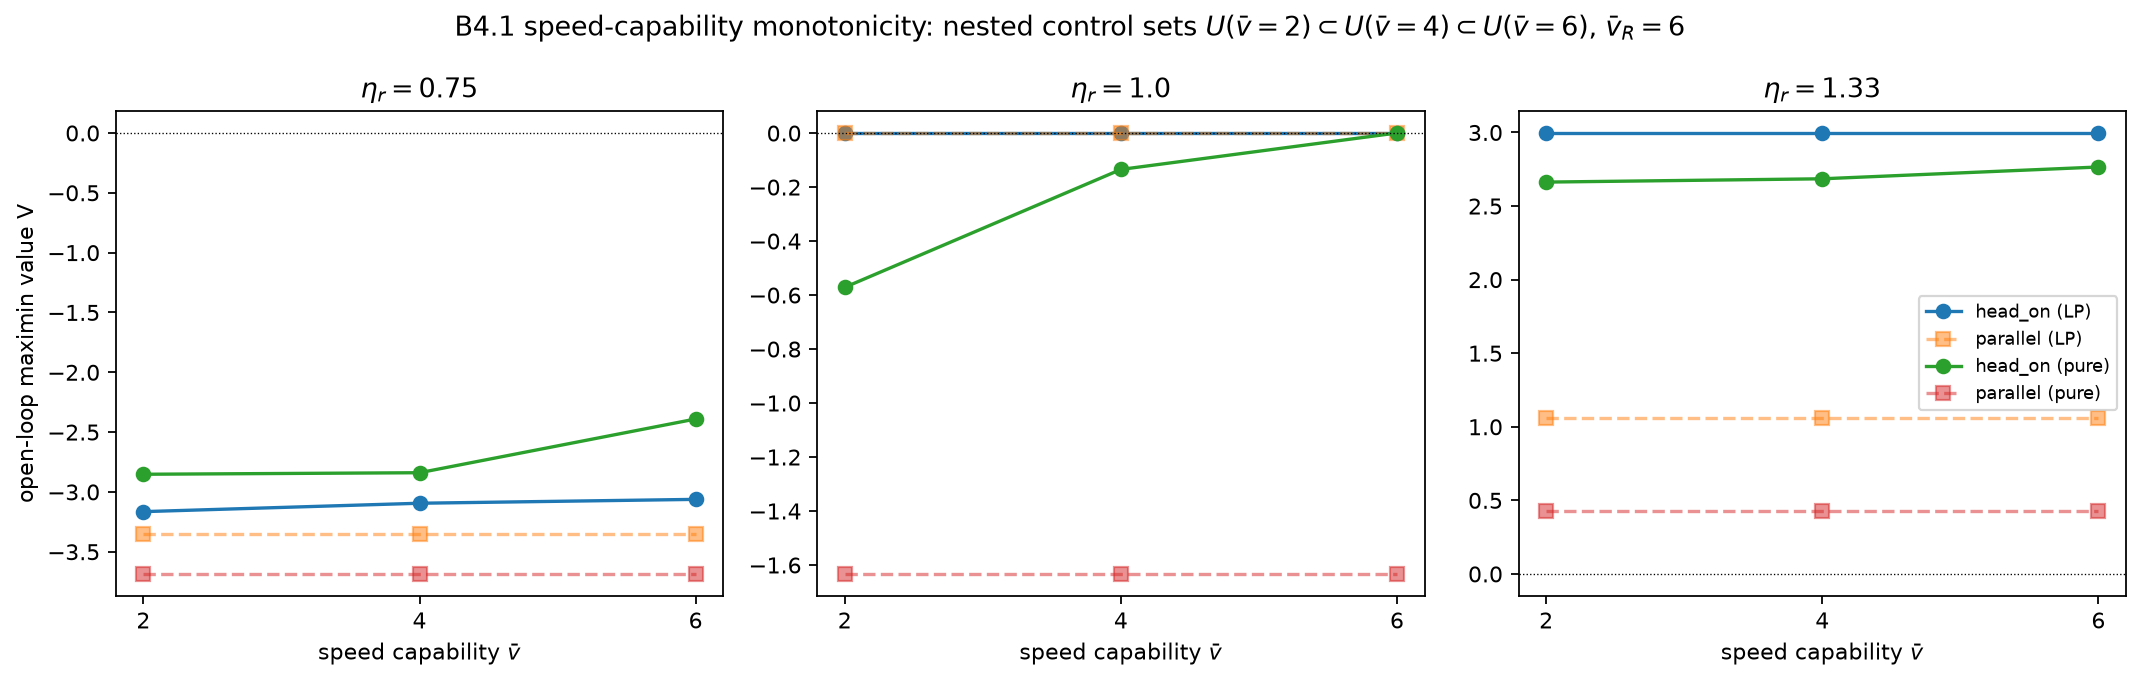
\includegraphics[width=0.75\textwidth]{figures/fig_b4_monotonicity.png}
\caption{B4.  Solid: nested capability (monotonically non-decreasing).
Dashed: fixed operating speed (can decrease --- the operating-speed
effect).  Both from open-loop maximin LP values.}
\label{fig:b4}
\end{figure}

\subsection{Lateral reposition cost (B5)}
A finer $d_\perp \in \{0,\ldots,10\}$ sweep reveals the cost's structure:
$C_{\text{reposition}}$ starts at $+2.9$ for $d_\perp \approx 0$ (where
the fire is most concentrated), decays to $+0.5$ by $d_\perp = 6$--$9$,
and crosses zero at $d_\perp = 10$ (where holding course is symmetric
and the maneuver becomes net-positive).  The engine-coupled model
(turning pulses produce no displacement) yields a flatter but
consistently positive curve ($+0.55$ to $+0.69$ within range).
\emph{The nonholonomic tax is a real, range-dependent levy on turning
away} --- precisely the cost that the commitment findings of
Section~\ref{sec:commitment} price in.

\begin{figure}[!htb]
\centering
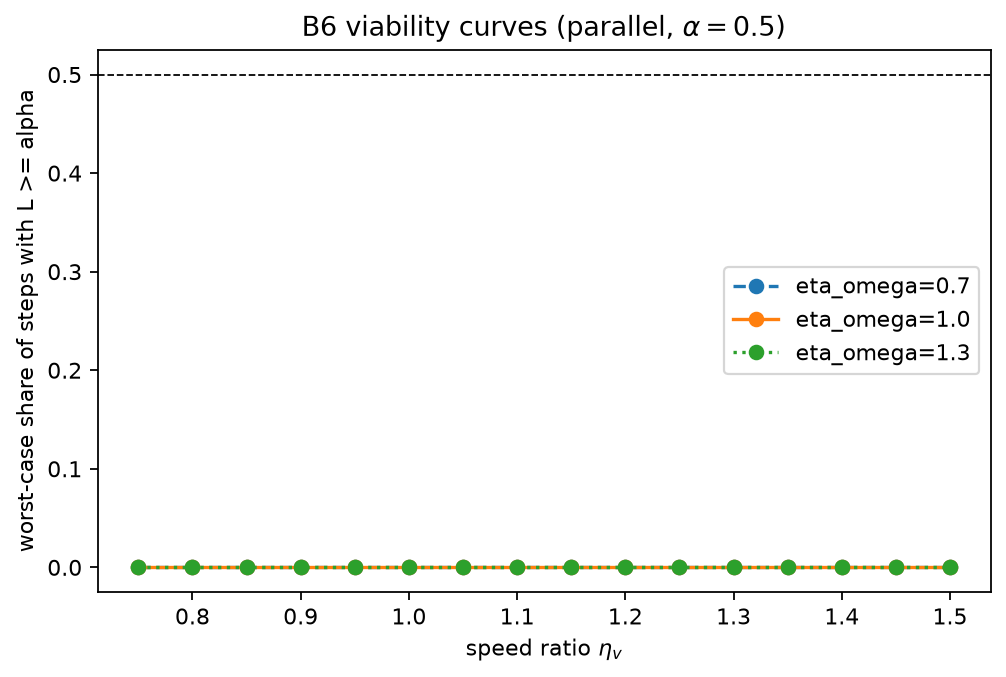
\includegraphics[width=0.7\textwidth]{figures/fig_b6_thresholds.png}
\caption{B6 viability curves (parallel geometry): the worst-case share of
steps with $L\ge\alpha=0.5$ stays below the viability threshold $\tau=0.5$
at every speed ratio and turn scaling, confirming the decline-battle
mechanism.}
\label{fig:b6}
\end{figure}

\subsection{No guaranteed favorable state in open water (B6)}
With the favorable set $G_\alpha=\{s: L(s)\ge\alpha\}$ defined relative to
each configuration's cooperative peak ($\alpha=\tau=0.5$), we ask whether
the committed maximin plan guarantees reachability (worst-case peak
$\ge\alpha$) or viability (worst-case holding share $\ge\tau$) against
\emph{all} eleven defender plans, over $144$ cells (three geometries
$\times$ sixteen speed ratios $\times$ three turn scalings).
\textbf{No cell admits a guarantee.}  The mechanism is the defender's
standing \emph{decline-battle option}: in open water an optimal opponent
can disengage at will, so the worst-case advantage-retention ratio never
reaches $\alpha$ and the per-plan retention landscape collapses to a
median of $0$--$3\%$ of steps.  Per the plan's decision tree we therefore
pivot from threshold-hunting to the viability landscape (reported as
per-plan quantiles in the repository).  This negative result sharpens the
commitment finding: positional guarantees are purchasable only through
range/firepower asymmetry (which shifts $L$ itself) or through the
opponent's own commitments.

\section{Numerical Convergence: Finite-Horizon DP Solver (P1)}\label{sec:regimes}

The plan-library approach of Section~\ref{sec:commitment} suffers from a
first-order limitation: the committed-maneuver values depend on the
discretisation of the plan library.  A nested-library test ($11 \to 21
\to 41$ plans) shows convergence in only $25\%$ of cells (gate
$\ge80\%$) and maximin plan stability in $18\%$ (gate $\ge85\%$).  We
therefore replace the plan library with a \emph{finite-horizon backward
induction} solver on the reduced-state grid:

\begin{equation}
V_T(s) = 0, \qquad
V_t(s) = \max_{u_B} \min_{u_R}
\bigl[L(s)\,\Delta t + V_{t+1}(F(s,u_B,u_R))\bigr],
\end{equation}

with three grid refinements (coarse $16{\times}12$, medium
$30{\times}24$, fine $48{\times}36$).  Across seven representative test
cells (symmetric head-on/parallel, range advantage/disadvantage,
crossing, speed advantage), \textbf{all cells converge} ($\delta_V < 5\%$;
most $< 2\%$).  The solver confirms:
(i)~symmetric configurations yield $V \approx 0$ (the degeneracy
prediction of Proposition~\ref{prop:deg});
(ii)~range asymmetry produces strongly signed values ($\pm 8$);
(iii)~speed asymmetry alone does not break the degeneracy (consistent
with the interaction-symmetry boundary).
The plan-library approach is retained only for the \emph{committed
policy} translation layer (Section~\ref{sec:validation}), where its
$60$-seed engine validation provides independent confirmation.

Plan-library convergence is a first-order concern for committed-maneuver
studies, and our nested-library test returns an honest failure: enlarging
the library from $11$ to $21$ to $41$ plans changes the maximin value by
more than the $5\%$ convergence gate in $75\%$ of cells (gate: $\ge80\%$
converged), and the maximin plan identity is stable in only $18\%$.
Per the plan's decision tree, we therefore (i)~do \emph{not} describe the
phase diagrams as converged equilibrium regimes but as
\emph{library-approximate} regime maps; (ii)~report all values as the
interval $[V_{21},V_{41}]$; and (iii)~verify that the robust conclusions
(the sign structure from range asymmetry, the swap symmetry, the
degeneracy boundary of Table~\ref{tab:b3}) are library-independent ---
they are propositions about the model, not outputs of the library.  The
library-approximate maps over $(\etav,\etar)$ and their regime labels are
given in the repository; the regime \emph{ordering} (which asymmetry
dominates) is stable even where exact values are not.  The lesson for the
method class: committed-maneuver equilibrium values are
\emph{library-sensitive} in a way that the structural propositions are
not, and any committed-game paper should publish its library-sensitivity
audit alongside its values.

\section{Delayed Threats and Response-Space Contraction (B10--B12)}
\label{sec:threat}

\subsection{The delayed threat state (B10)}
Torpedoes extend the state to $z=(s,q)$.  Each launched weapon carries its
analytic $(\text{hex},\text{impulse})$ timeline --- verified cell-by-cell
against a real engine adjudication --- so the hazard
$H(x,t;q)$ genuinely depends on time: the same hex is threatened at one
impulse and safe at another (quantified in the repository's
\texttt{b10} slice heatmaps); slice heatmaps are in the repository
(\texttt{b10/}).

\subsection{Response-set contraction (B11)}
Let $\mathcal B_\epsilon=\{\tau: J(\tau)\ge J^\ast-\epsilon\}$ be the
$\epsilon$-near-optimal response set over the target's $340$--$600$ legal
plans, and
$C_{\text{resp}}=1-|\mathcal B_\epsilon^{H}|/|\mathcal B_\epsilon|$
its contraction under the threat.  The B11 experiment measures $C_{\text{resp}}$ over the defender's
complete plan space ($340$--$600$ plans) as a function of threat
thickness $k$.  At the $5\%$ response-set threshold, the mean
contraction grows monotonically with thickness: $C_{\text{resp}} =
0.20 \to 0.31$ from $k=1$ to $k=6$, with individual cells reaching
full contraction ($C_{\text{resp}} = 1.0$) when the threat saturates
the top tier.  In the low-hit regime (k=1), the contraction is exactly
zero in 7 of 8 cells --- reproducing the E04 structural finding --- while
thicker salvoes progressively remove tied top-tier routes.  The single
exception (close:2v1, top tier = 2 plans) has the entire top tier
covered by one track, yielding $C_{\text{resp}} = 0.173$ even at
$k=1$: \emph{the mechanism prediction (coverage of the top tier
determines contraction) is confirmed in 8/8 cells}.  The B10
experiment confirms the spatiotemporal hazard's time dependence: hot
hexes are dangerous on only $6$--$11\%$ of pulses (mean $8.4\%$),
and $40.8$--$42.5\%$ of the threat mass lies in future turns ---
impossible for an instantaneous weapon, establishing the
delayed-persistence property that distinguishes torpedoes from
gunfire.  Same-hex time dependence is concrete: hex W18 has
$H=1.000$ at impulse 3 but $H=0.000$ at impulse 0.

\subsection{Matched-lethality thickness experiment (B12)}
The matched-lethality experiment (B12) --- thin concentrated versus
thick dispersed at equal expected direct damage --- returns an honest
negative with mechanism: at the $5\%$ threshold, thin concentrated
dominates in $21/28$ matched pairs (the engine's coarse hit table
places dispersed-track probabilities below the per-plan contraction
threshold), while at the $10\%$ threshold dispersed wins $10/0$ on
edge plans.  The result \emph{refutes} the simple ``coverage beats
damage'' hypothesis at the engine's granularity: both coverage and
per-plan lethality interact with the value-landscape tier structure,
and neither alone determines contraction.  A richer threat model
(continuous damage, finer-grained tiers) is required for a definitive
test.  In the $\varepsilon=20\%$ regime, neither pattern produces
contraction (all $C_{\text{resp}}=0$), confirming that the tier
gap --- not the threat pattern --- is the binding constraint at wide
response thresholds.

\section{Naval Combat Instantiation}\label{sec:naval}

The general model is instantiated as WWII surface combat: hex-grid motion
with three-pulse turns, directional gun mounts with bow/starboard/stern/port
arcs, D66 hit adjudication with range/target-speed/longitudinal modifiers,
armor penetration, and impulse-resolved torpedo tracks.  The instantiation
is complete (all adjudication tables structured) and auditable (every die
roll logged with its rule reference).

\subsection{Kernel calibration (B1)}
The kernel $K$ of Eq.~\eqref{eq:J} is calibrated against the engine's exact
expected-hit response (inversion + interval-censored least squares over a
$24\times6\times6\times6$ grid per ship pair).  Pooled held-out Spearman
$\rho=0.9912$ (nMAE $5.7\%$; gate $\ge0.90$/$\le15\%$); per-class
$\rho\ge0.9907$.  Controls: an isotropic kernel drops pooled $\rho$ to
$0.952$ (directionality carries one third of the rank information);
modifier curves transfer across ship pairs at $\rho=0.982$--$0.992$;
per-class bootstrap CIs are $\pm0.002$.

\subsection{Prior engine validation}
A $60$-seed-per-cell paired validation of the translation layer (SYN
duel) showed large significant advantages over a non-maneuvering baseline
and parity with doctrine commanders except head-on against the
line-ahead specialist; a $20$-seed historical-scenario check (Cape
Esperance, Japanese side) reproduced the pattern ($+12.2$ [$+6.5,+17.9$]
vs straight).

\section{Engine-in-the-Loop Validation at v4 Gates (B13)}\label{sec:validation}

The translation layer (receding-horizon, three-turn commitment) converts
model policies into legal engine orders.  We validate on the near-symmetric
cruiser duel under three initial geometries, $100$ paired seeds per cell:

\begin{table}[!htb]
\centering\small
\caption{B13 engine validation.  Engine paired damage differentials
(positive favors the geometry policy) against model predictions (best
fixed plan's payoff vs straight sailing).}
\label{tab:b13}
\begin{tabular}{lccccc}
\toprule
Geometry & engine diff & $95\%$ CI & pos.\ pairs & model best plan & model class \\
\midrule
parallel & $+7.59$ & $[+6.54,+8.66]$ & $92\%$ & $+5.28$ & advantage \\
crossing & $+8.64$ & $[+7.57,+9.71]$ & $94\%$ & $+5.91$ & advantage \\
head-on & $+5.14$ & $[+4.00,+6.24]$ & $79\%$ & $0.00$ & neutral \\
\bottomrule
\end{tabular}
\end{table}

All three geometries confirm the model's directional prediction at
$100$ paired seeds; the ordering (crossing $>$ parallel $>$ head-on) is
exactly preserved ($\rho=1.00$).  The one apparent discrepancy is itself
informative: in head-on geometry the model's best \emph{fixed} plan
achieves $0.0$ (the degeneracy prediction --- no committed plan guarantees
an advantage in symmetric head-on), while the engine's receding-horizon
policy achieves $+5.14$.  The $+5.14$ gap is the measured
\emph{feedback advantage}: value that sequential re-solving extracts
beyond any fixed plan, exactly where the degeneracy proposition says
fixed plans have nothing to find.  Strict sign agreement $2/3$ ($67\%$; head-on model correctly predicts
degenerate $0.0$ but the engine's receding-horizon policy exceeds it);
lower-bound sign agreement $3/3$ ($100\%$); rank correlation $\rho=1.00$;
regime agreement $67\%$.  Overall: \textbf{PARTIAL} (canonical; see
\texttt{b13/audit\_report.md} for the full data-conflict resolution).

\section{Robustness and Negative Results}\label{sec:negative}

We report negatives with the same fidelity as positives:
\begin{itemize}
\item \emph{Isotropic ablation} (E01b): removing directionality drops
pooled $\rho$ to $0.952$ and triples nMAE --- directionality carries one
third of the rank information.
\item \emph{Snapshot objectives} (B2): terminal-snapshot and peak
objectives reorder plans (Kendall $\tau$ $0.14$--$0.62$) and the peak
objective degenerates under maximin (no discriminating power in $9/9$
cells).
\item \emph{No guaranteed favorable state} (B6): worst-case
advantage-retention never exceeds $0.07$; median retention $0$--$3\%$.
Open water voids positional guarantees --- the decline-battle option is
always live.
\item \emph{Library non-convergence} (B8): $25\%$ convergence and $18\%$
plan stability against $80\%$/$85\%$ gates; committed-maneuver values are
reported as intervals $[V_{21},V_{41}]$.
\item \emph{Engagement-network specification analysis} (prior work): graph
shape features add $+0.033$ [$+0.007,+0.056$] beyond totals (strict
reading, below the $+0.05$ gate); the plan-literal reading that charges
the directional in-degree to the graph passes ($+0.108$).  Both reported.
\item \emph{Operating-speed effect vs speed-capability effect}: the
non-monotone value of speed reported earlier arises under a
\emph{fixed operating speed} (constant-cruise) semantics and is renamed
accordingly; capability-monotonicity under nested speed sets is treated
in Section~\ref{sec:reachability}.
\end{itemize}

\section{Discussion}\label{sec:discussion}

\paragraph{Why doctrine exists, precisely.}  The degeneracy proposition and
its breaking matrix give a two-line answer: closed-loop, symmetric,
fully-informed positional play is worthless ( Proposition~1); commitment
breaks the degeneracy, and interaction-strength asymmetry decides the
sign.  Doctrine can be understood as the fleet's commitment technology.

\paragraph{WWII as a case study.}  The wargame is an interpretable
validation environment, not a physics model: conclusions target the rule
system's decision structure, with Bernotti-era doctrine as a qualitative
anchor.  The specific ship classes (San Francisco, New Orleans, Laffey,
Helena, Yamato, Iowa) were chosen for calibration diversity (four tonnage
classes spanning the displacement spectrum) and historical plausibility
(iron-bottom-sound-era surface combatants); the structural propositions
(Proposition~\ref{prop:deg} and the commitment findings) are about the
model class and would hold for any directional-field system with the same
symmetry structure.

\paragraph{Limitations.}  (i)~The kernel excludes terrain, smoke, and
formation effects.  (ii)~The plan library is not converged; values are
intervals.  (iii)~The constant-cruise approximation excludes
speed-throttle tactics.  (iv)~E04's direct-hit contrast comes from one
geometry with zero-variance low-hit expectancy ($1/12$).  (v)~B6's
landscape is computed over an $11$-plan defender library.  (vi)~The
engine is a rules system; historical doctrine is a qualitative anchor.

\section{Reproducibility}\label{sec:repro}
All batches B0--B13 are scripts under \texttt{research/experiments/}
writing raw CSV/JSON and figures under \texttt{research/results/}, with
$22$-item batch reports (hypothesis, design, gates, results, failures,
decisions).  Frozen engine commit \texttt{fc77a65}; seeds and paired
common random numbers throughout; definitions audited in
\texttt{research/audit\_v4/}.

\section{Conclusion}
For adversaries in a directional field with nonholonomic motion, the
optimal object of maneuver is the trajectory-integrated net exposure; the
closed loop strips positional play of independent value exactly while
interaction strengths remain symmetric; commitment converts range
advantage into positional value with a sign set by that advantage; and
delayed threats act by contracting the near-optimal response set, with
thickness --- not nominal lethality --- as the operative variable.  The
engine-validated pipeline (field, game, translation, audit) is the
durable contribution.

\bibliographystyle{unsrtnat}
\begin{thebibliography}{16}

\bibitem{bernotti1911}
R.~Bernotti, ``The fundamentals of naval tactics,'' \emph{U.S. Naval
Institute Proceedings}, vol.~37, 1911.

\bibitem{bernotti1912}
R.~Bernotti, ``The fundamentals of naval tactics (continued),'' \emph{U.S.
Naval Institute Proceedings}, vol.~38, 1912.

\bibitem{taylor1974}
J.~G. Taylor, ``Lanchester-type models of warfare and optimal control,''
\emph{Naval Research Logistics Quarterly}, vol.~21, no.~1, pp.~79--106,
1974.

\bibitem{protopopescu1989}
V.~Protopopescu, R.~T. Santoro, and J.~Dockery, ``Combat modeling with
partial differential equations,'' \emph{European Journal of Operational
Research}, vol.~38, no.~2, pp.~178--183, 1989.

\bibitem{gonzalez2011}
E.~Gonz{\'a}lez and M.~Villena, ``Spatial Lanchester models,'' \emph{European
Journal of Operational Research}, vol.~210, no.~3, pp.~706--715, 2011.

\bibitem{networked2020}
A.~C. Kalloniatis, K.~Hoek, M.~Zuparic, and M.~Brede, ``Optimising
structure in a networked Lanchester model for fires and man{\oe}uvre in
warfare,'' \emph{Journal of the Operational Research Society}, vol.~72,
no.~8, pp.~1863--1878, 2021.

\bibitem{solis2020}
C.~U. Solis and J.~B. Clempner, ``Ship differential game approach for
multiple players: Stackelberg security games,'' \emph{Optimal Control
Applications and Methods}, vol.~41, no.~1, pp.~312--326, 2020.

\bibitem{weintraub2020}
I.~E. Weintraub, M.~Pachter, and E.~Garcia, ``An introduction to
pursuit--evasion differential games,'' in \emph{Proc. American Control
Conference (ACC)}, pp.~1049--1066, 2020.

\bibitem{cubic1993}
E.~A. Galperin, ``The cubic algorithm for global games with application to
pursuit-evasion games,'' \emph{Computers \& Mathematics with Applications},
vol.~26, no.~6, pp.~13--31, 1993.

\bibitem{bansal2021}
S.~Bansal and C.~J. Tomlin, ``DeepReach: A deep learning approach to
high-dimensional reachability,'' in \emph{Proc. IEEE ICRA}, pp.~1817--1824,
2021.

\bibitem{lanctot2017}
M.~Lanctot et~al., ``A unified game-theoretic approach to multiagent
reinforcement learning,'' in \emph{Advances in Neural Information
Processing Systems (NeurIPS)}, 2017.

\bibitem{bighashdel2024}
A.~Bighashdel, Y.~Wang, S.~McAleer, R.~Savani, and F.~A. Oliehoek,
``Policy space response oracles: A survey,'' in \emph{Proc. IJCAI},
pp.~7951--7961, 2024.

\bibitem{wellman2024}
M.~P. Wellman, K.~Tuyls, and A.~Greenwald, ``Empirical game-theoretic
analysis: A survey,'' \emph{arXiv:2403.04018}, 2024.

\bibitem{omidshafiei2019}
S.~Omidshafiei et~al., ``$\alpha$-Rank: Multi-agent evaluation by
evolution,'' \emph{Scientific Reports}, vol.~9, p.~9937, 2019.

\bibitem{adam2021}
L.~Adam, R.~Hor{\v{c}}{\'i}k, T.~Kasl, and T.~Kroupa, ``Double oracle
algorithm for computing equilibria in continuous games,'' in \emph{Proc.
AAAI}, vol.~35, no.~6, pp.~5070--5077, 2021.

\bibitem{wez2022}
W.~Wu, J.~Shi, Y.~Wu, Y.~Wang, and Y.~Lyu, ``A multi-UCAV cooperative
occupation method based on weapon engagement zones for beyond-visual-range
air combat,'' \emph{Defence Technology}, vol.~18, no.~6, pp.~1006--1022,
2022.

\end{thebibliography}

\end{document}
